\section{Neutral case}
In this section, we assume that the stratification is neutral.
There is no effect of the stratification on the turbulent viscosity
so the wind speed $u(z, t)$ can be integrated in time
without the temperature and humidity profiles.
We first present the continuous model used and its
discretization with finite volumes. Several strategies to
take into account the surface layer are then presented.
\subsection{Continuous model and Finite Volumes discretization}
\subsubsection{Continuous equations: two separate domains}
\label{sec:ND_NeutralCase}
The continuous equation above the surface layer
($z > \delta_{\rm sl}$) is
\begin{equation}
	\label{eq:ND_NeutralCase_EkmanEq}
  (\partial_t + if) u - \partial_z (K_u \partial_z u) = if u_G
\end{equation}
where $u_G$ is a constant value representing the geostrophic guide.
$f$ is the Coriolis parameter and $K_u$ the turbulent viscosity.
The profile of $K_u$ will be detailed
in section \ref{sec:ND_StratifiedCase_turbulentVisc}.
inside the surface layer ($z \leq \delta_{\rm sl}$), the flux
$K_u \partial_z u$ is constant:
\begin{equation}
	\label{eq:ND_NeutralCase_constantFlux}
	\left.K_u \partial_z u \right|_{z\leq \delta_{\rm sl}}
	= u_\star^2
	\frac{u(\delta_{\rm sl}, t)}{||u(\delta_{\rm sl}, t)||}.
\end{equation}
The size of the turbulent eddies at height $z$
is proportional to the distance to the surface $z$
(e.g. \cite{kawai2012wall}). Combining molecular and
turbulent viscosities gives 
$K_u(z\leq \delta_{sl}) = \kappa u_\star z + K_{u, {\rm mol}}
= \kappa u_\star (z + z_{0M})$ with $z_{0M} = \frac{K_{u, {\rm mol}}}{\kappa u_\star}$.
It follows that
\begin{equation}
\label{eq:ND_NeutralCase_WallLaw}
	||u(z, t) - u(0, t)|| = \frac{{u_\star}}{\kappa}
	\log(1+\frac{z}{z_{0M}}).
\end{equation}
A typical integration in time from $u(z, t^{n})$ to
$u(z, t^{n+1})$ is:
\begin{enumerate}
  \item Use \eqref{eq:ND_NeutralCase_WallLaw} to compute 
	  $u_\star = \frac{\kappa ||u(z, t^n)||}
			{\log(1+\frac{z}{z_{0M}})}$
  \item Integrate in time \eqref{eq:ND_NeutralCase_EkmanEq}
  using \eqref{eq:ND_NeutralCase_constantFlux} as a boundary condition
		either of Neumann type ($\left.K_u \partial_z u
		\right|_{z\leq \delta_{\rm sl}, t^{n+1}}
	= u_\star^2 \frac{u(\delta_{\rm sl}, t^n)}
		{||u(\delta_{\rm sl}, t^n)||}$)
		or of Robin type ($\left.K_u \partial_z u
		\right|_{z\leq \delta_{\rm sl}, t^{n+1}}
		- \frac{u_\star^2} {||u(\delta_{\rm sl}, t^n)||}
		u(\delta_{\rm sl}, t^{n+1}) = 0$)
\end{enumerate}

\subsubsection{Discretization with Finite volumes}
We define here the discretization used throughout all the present
section. The space domain is divided into $M$ cells delimited by
heights $(z_0=0, .., z_m, .., z_M)$. The size of the $m$-th cell
is $h_{m-\frac{1}{2}}=z_{m}-z_{m-1}$ and the average of $u(z, t)$
over this cell is 
$\overline{u}_{m-\frac{1}{2}}=\frac{1} {h_{m-\frac{1}{2}}}
\int_{z_{m-1}}^{z_m}u(z, t)dz$.
The space derivative of $u$ at $z_m$ is noted $\phi_{m}$.
Averaging \eqref{eq:ND_NeutralCase_EkmanEq} over a cell gives
the semi-discrete equation
\begin{equation}
\label{eq:ND_NeutralCase_semiDiscreteEkmanEq}
	(\partial_t + if) \overline{u}_{m+\frac{1}{2}} - 
	\frac{K_{u, m+1} \phi_{m+1} - K_{u, m} \phi_{m}}
		{h_{m+\frac{1}{2}}} = i f u_G.
\end{equation}
The reconstruction of $u(z, t) = {\cal S}_{m+\frac{1}{2}}
				(z - z_{m+\frac{1}{2}})$
				inside a cell must be decided
to pursue the derivation of the scheme. The simplest choice is
a quadratic polynomial,
${\cal S}_{m+\frac{1}{2}}(\xi) = r_0 + r_1 \xi + r_2 \xi^2$ where
$-\frac{h_{m+1/2}}{2} \leq \xi \leq \frac{h_{m+1/2}}{2}$.
Averaging ${\cal S}_{m+\frac{1}{2}}$ over the cell and
prescribing its space derivative at $z_{m}$ and $z_{m+1}$
($\xi=-\frac{h_{m+\frac{1}{2}}}{2}, \frac{h_{m+\frac{1}{2}}}{2}$)
lead to the following system:
\begin{equation}
    \begin{pmatrix}
    \overline{u}_{m+1/2} \\
    h_{m+\frac{1}{2}} \phi_m \\
	    h_{m+\frac{1}{2}} \phi_{m+1}
    \end{pmatrix} = 
    \begin{pmatrix}
    1 & 0 & \frac{1}{12} \\
    0 & 1 & -1 \\
    0 & 1 & 1 \\
    \end{pmatrix}
    \begin{pmatrix}
    r_0 \\
    r_1 h_{m+\frac{1}{2}} \\
    r_2 h_{m+\frac{1}{2}}^2
    \end{pmatrix}
\end{equation}
The reconstruction of $u(z)$ between $z_m$ and $z_{m+1}$
is then
\begin{equation}
\label{eq:ND_NeutralCase_quadraticReconstruction}
{\cal S}_{m+\frac{1}{2}}(\xi) =
	\Bar{u}_{m+\frac{1}{2}} + 
	\frac{\phi_{m+1}^{} + \phi_{m}^{}}{2} \xi
	+ \frac{\phi_{m+1}^{} - \phi_{m}^{}}{2h_{m+1/2}}
	\left(\xi^2 - \frac{h_{m+1/2}^2}{12}\right).
\end{equation}

The continuity of the solution at cell interfaces (${\cal S}_{m-\frac{1}{2}}\left(\frac{h_{m-1/2}}{2}\right) = {\cal S}_{m+\frac{1}{2}}\left(-\frac{h_{m+1/2}}{2}\right)$) is equivalent to
%
\begin{equation}
\label{eq:ND_NeutralCase_continuityEquationFV}
\frac{h_{m-1/2}}{6} \phi_{m-1} 
+ \frac{2h_{m}}{3} \phi_m  
+ \frac{h_{m+1/2}}{6} \phi_{m+1} = \Bar{u}_{m+\frac{1}{2}} - \Bar{u}_{m-\frac{1}{2}}
\end{equation}
where $h_m = \frac{h_{m-1/2} + h_{m+1/2}}{2}$.
Combining \eqref{eq:ND_NeutralCase_semiDiscreteEkmanEq}
and \eqref{eq:ND_NeutralCase_continuityEquationFV} finally gives
the prognostic equation to integrate
$\partial_z u$ in time:
\begin{equation}
\begin{aligned}
\label{eq:ND_NeutralCase_prognosticEqFV}
(\partial_t + if) \left( \frac{h_{m-1/2}}{6h_m} \phi_{m-1} 
+ \frac{2}{3} \phi_m  
+ \frac{h_{m+1/2}}{6h_m} \phi_{m+1} \right)& \\
-
    \left(
	\frac{K_{u, m+1}}{h_m h_{m+1/2}}\phi_{m+1} - \frac{2 K_{u,m}}{h_{m-1/2} h _{m+1/2}}\phi_m + \frac{K_{u,m-1}}{h_m h_{m-1/2}}\phi_{m-1}
    \right)
&= 0
\end{aligned}
\end{equation}
To reconstruct the solution, $\overline{u}$ should also be 
integrated in time with \eqref{eq:ND_NeutralCase_semiDiscreteEkmanEq}.
\eqref{eq:ND_NeutralCase_prognosticEqFV} and
\eqref{eq:ND_NeutralCase_semiDiscreteEkmanEq} are hence the two 
equations defining our finite volumes discretization.

\paragraph{Fourth order compact scheme}
To get a more accurate scheme,
a fourth degree polynomial can also be used. If
${\cal S}_{m+\frac{1}{2}}^4(\xi) = r_0^4 + r_1^4 \xi + r_2^4 \xi^2 
+ r_3^4 \xi^3 + r_4^4 \xi^4$, we can recover a fourth order compact
scheme by putting as a constraint that the reconstruction
on the boundaries of the cell are
${\cal S}^4_{m+\frac{1}{2}}(\frac{h_{m+\frac{1}{2}}}{2}) =
\overline{u}_{m+\frac{1}{2}} + \frac{h_{m+\frac{1}{2}}}{12}\left(
\phi_m + 5\phi_{m+1}\right) $ and
${\cal S}^4_{m+\frac{1}{2}}(-\frac{h_{m+\frac{1}{2}}}{2}) =
\overline{u}_{m+\frac{1}{2}} - \frac{h_{m+\frac{1}{2}}}{12}\left(
5\phi_m + \phi_{m+1}\right)$.
Then the reconstruction is given by
\begin{equation}
    \begin{pmatrix}
    r_0^4 \\
    r_1^4 h_{m+\frac{1}{2}} \\
    r_2^4 h_{m+\frac{1}{2}}^2 \\
    r_3^4 h_{m+\frac{1}{2}}^3 \\
    r_4^4 h_{m+\frac{1}{2}}^4
    \end{pmatrix}
     = 
    \begin{pmatrix}
    1 & 0 & \frac{1}{12} & 0 & \frac{1}{80} \\
    0 & 1 & -1 & \frac{3}{4} & -\frac{1}{2} \\
    0 & 1 & 1 & \frac{3}{4} & \frac{1}{2} \\
    1 & -\frac{1}{2} & \frac{1}{4} & -\frac{1}{8}
    & \frac{1}{16} \\
    1 & \frac{1}{2} & \frac{1}{4} & \frac{1}{8}
    & \frac{1}{16} \\
    \end{pmatrix}^{-1}
    \begin{pmatrix}
    \overline{u}_{m+1/2} \\
    h_{m+\frac{1}{2}} \phi_m \\
	    h_{m+\frac{1}{2}} \phi_{m+1} \\
	    \overline{u} - \frac{5}{12} h_{m+\frac{1}{2}} \phi_m - \frac{1}{12} h_{m+\frac{1}{2}} \phi_{m+1} \\
	    \overline{u} + \frac{1}{12} h_{m+\frac{1}{2}} \phi_m + \frac{5}{12} h_{m+\frac{1}{2}} \phi_{m+1}
    \end{pmatrix}
\end{equation}

\subsection{Wall law}
We show here several strategies for the discretization
in the surface layer. We first compare 3 state-of-the-art
discretizations then introduce an original one.

The discretization consists in three parts:
\begin{itemize}
	\item How $u(\delta_{\rm sl}, t^n)$ is computed
		(which influence the value of $u_\star$);
	\item How the boundary condition 
		\eqref{eq:ND_NeutralCase_constantFlux} is implemented.
\end{itemize}
\subsubsection{State-of-the-art strategies}
  We now present three strategies that are representative of
  what is done in models. A summary of those discretizations
  is presented in Figure \ref{fig:ND_NeutralCase_summary_sfscheme}.
  \begin{itemize}
	  \item "FV pure": $\delta_{\rm sl} = z_{\frac{1}{2}}$. Similar to a Finite Differences discretization.
	    The reconstruction of $u(z)$ is used to get 
		  $u(z_{\frac{1}{2}})$.
		  The first cell is treated like the others
		  (i.e. \eqref{eq:ND_NeutralCase_EkmanEq} is
		  applied inside the surface layer).
	The bottom boundary condition is 
		  $ K_{u,0} \phi_0^{n+1} = u_\star^2 
		  \frac{{\cal S}_{1/2}^{n+1}(0)}{||{\cal S}_{1/2}^n(0)||}$.
	  \item "FV1": $\delta_{\rm sl} = z_{\frac{1}{2}}$.
		  In state-of-the-art models using finite volumes,
		  $u_{\star}$ is often computed using
		  $u(\delta_{sl}) = \overline{u}_{\frac{1}{2}}$
		\cite{nishizawa2018surface}.
		The corresponding bottom boundary condition is
		$ K_{u,0} \phi_0^{n+1} = u_\star^2 
		  \frac{\overline{u}^{n+1}_{\frac{1}{2}}}
		  	{\overline{u}_{\frac{1}{2}}^n}$.

    \item "FV2":  $\delta_{\rm sl} = z_{1}$. In
    \cite{nishizawa2018surface}, the "FV1" strategy is shown to systematically
	  underestimate $u(\delta_{\rm sl})$ because of the 
	  convexity of the logarithmic profile.
	A surface flux scheme is derived by assuming
	  $\delta_{\rm sl} = z_1$ and by integrating $u(z)$
	  in space in the first cell. Since the reconstruction
	  of $u(z)$ is continuous, it is here equivalent to
	  get $u_\star$ through
	  $u^n(\delta_{\rm sl}) = {\cal S}^n_{\frac{3}{2}}(
	  -\frac{h_{3/2}}{2})$. The first cell is only
	  parametrized with the wall law, and the boundary condition
		  at $z_1$ is $K_{u,1} \phi_1 - u_\star^2 
		  \frac{{\cal S}_{\frac{3}{2}}^{n+1}
		  	(-h_{\frac{3}{2}}/2)}
		  {||u^n(\delta_{\rm sl})||} = 0$
	  
  \end{itemize}
  Note that for the first two strategies, $K_{u,0}$
  should not actually
  take the value $\left. K_{u}\right|_{z=0}$.
  See section \ref{sec:ND_StratifiedCase_viscosity0_FVpure} for
  the explanation.

\begin{figure}
	\centering
	\subimport{images/}{sf_scheme_strategies.pdf_tex}
	\caption{Summary of the surface flux schemes. The
	wind profiles shown here do not correspond to
	numerical values.}
	\label{fig:ND_NeutralCase_summary_sfscheme}
\end{figure}

The "FV pure" and "FV1" strategies are not satisfactory because
\begin{itemize}
	\item "FV1" relies on the assumption that $\overline{u}_{\frac{1}{2}} = u(z_{\frac{1}{2}})$
	\item both strategies assume that $u(z)$ is a parabolic spline in the surface layer and that $\eqref{eq:ND_NeutralCase_EkmanEq}$
		can be applied as well.
\end{itemize}
The "FV2" surface flux scheme solves those problems.
However, for all those discretizations, changing the space step
also changes the height of the surface layer $\delta_{\rm sl}$.
In the following, we derive a surface flux scheme that keep
the advantages of the "FV2" with a free $\delta_{\rm sl}$.

\subsubsection{A surface flux scheme with a free $\delta_{\rm sl}<z_1$}
We now construct a boundary condition that is coherent
with the wall law with a free $\delta_{sl}$. We first assume
that $\delta_{\rm sl} < z_1$ and then relax this hypothesis.
In the first grid level, we assume that
\eqref{eq:ND_NeutralCase_WallLaw} applies for $z<\delta_{sl}$
which leads us to separate the 
first volume into two parts: the surface layer $[0,\delta_{\rm sl}]$ and the "subcell" $[\delta_{\rm sl}, z_1]$ of size $\widetilde{h}$, of average $\widetilde{u}$
and of subgrid reconstruction
${\cal S}_{1/2}(\xi) = \widetilde{u} + \frac{\phi_{1} + \phi_{0}}{2} \xi
+ \frac{\phi_{1} - \phi_{0}}{2\widetilde{h}}\left(\xi^2 - \frac{\widetilde{h}^2}{12}\right)
$.
Here, $\xi = z - (z_1 - \frac{\widetilde{h}}{2})$.
The relation between $\overline{u}_{1/2}$ and $\widetilde{u}$ is 
\begin{equation}
\label{eq:ND_NeutralCase_Chasles}
	\widetilde{h}\widetilde{u} = h_{1/2}\overline{u}_{1/2} - \frac{u^{n+1}(\delta_{sl})}{||u^n(\delta_{sl})||}\frac{{u_\star}}{\kappa}\int_{z_0}^{\delta_{sl}} \log(1+\frac{z}{z_{0M}}) dz.
\end{equation}
The notations are summed up in Figure
\ref{fig:ND_NeutralCase_nouvelle_dis_neutre}.
The time indices of $\frac{u^{n+1}(\delta_{sl})}{||u^n(\delta_{sl})||}$
in \eqref{eq:ND_NeutralCase_Chasles} directly come from the integration 
of $\partial_z u$ given by the Robin boundary
condition \eqref{eq:ND_NeutralCase_constantFlux}.
\begin{figure}
	\subimport{images/}{nouvelle_dis_neutre.pdf_tex}
	\caption{Surface layer scheme "FV free"}
	\label{fig:ND_NeutralCase_nouvelle_dis_neutre}
\end{figure}


Let us inject $u(\delta_{sl}) = \widetilde{u} - \widetilde{h}(\phi_0/3 + \phi_1/6)$ and $||u(\delta_{sl})|| = \frac{{u_\star}}{\kappa}\log(1+\frac{\delta_{sl}}{z_{0M}})$:
\begin{equation}
\frac{\widetilde{h}}{h_{1/2}}\widetilde{u} = \overline{u}_{1/2} - \tau_{sl}\left(\widetilde{u} - \widetilde{h}(\phi_0/3 + \phi_1/6)\right).
\end{equation}
with $\tau_{sl} = \frac{1}{{h_{1/2}}}\int_{z_0}^{\delta_{sl}} \frac{\log(1+\frac{z}{z_{0M}})}{\log(1+\frac{\delta_{sl}}{z_{0M}})} dz =
\frac{(\delta_{\rm sl} + z_{0M})\log(1+\frac{\delta_{\rm sl}}{z_{0M}}) - \delta_{\rm sl}}{h_{1/2}\log(1+\frac{\delta_{sl}}{z_{0M}})}$ a non-dimensional number $0 \leq\tau_{sl} < 1$. (In this neutral case $\tau_{\rm sl} = 0 \iff \widetilde{h}=h_{1/2}$)

\paragraph{Evolution of $\tau_{\rm sl}$}
$\tau_{\rm sl}$ is a constant in the neutral case
when $\delta_{\rm sl}$ and $z_{0M}$ are constants. However,
$z_{0M}$ depends on $u_\star$ and will vary.
In all this document we assume that $\delta_{\rm sl}$ is a constant.

Let $\alpha_{\rm sl} = \frac{\widetilde{h}}{h_{1/2}}+\tau_{sl}$.
Then $\widetilde{u} = \frac{1}{\alpha_{\rm sl}}\left(\overline{u}_{1/2} + \widetilde{h}\tau_{sl}(\phi_0/3 + \phi_1/6)\right)$
and $u(\delta_{sl})=\frac{\overline{u}_{1/2} - \frac{\widetilde{h}^2}{h_{1/2}}
(\frac{\phi_0}{3} + \frac{\phi_1}{6})}{\alpha_{\rm sl}}$.
The scheme can then use as boundary condition:
\begin{equation}
	\label{eq:ND_NeutralCase_boundaryCondFVfree}
	K_{u,0} \phi_0 = {u_\star}^2
	\frac{\overline{u}_{1/2} - \frac{\widetilde{h}^2}{h_{1/2}}(\frac{\phi_0}{3} + \frac{\phi_1}{6})}{\alpha_{\rm sl}^{n+1}||u^n(\delta_{sl})||}
\end{equation}

Similarly to \eqref{eq:ND_NeutralCase_continuityEquationFV}
the continuity of the subgrid reconstruction at $z_1$ requires that
\begin{equation}
	\label{eq:ND_NeutralCase_continuityFVfree}
    \frac{\widetilde{h}}{6} 
    \phi_0
    +
    (\frac{\widetilde{h}}{3} 
    + \frac{h_{3/2}}{3})
    \phi_1
    + \frac{h_{3/2}}{6} \phi_2
     = \overline{u}_{3/2} - 
     \widetilde{u}.
\end{equation}
Finally, the scheme at the first grid level is
\begin{equation}
	\label{eq:ND_NeutralCase_prognosticEqFVfree}
    \begin{aligned}
(\partial_t + if)
    \left(\frac{\widetilde{h}}{6h_1} 
    \phi_0
    +
    \left(
    \frac{\widetilde{h}}{3h_1} 
    + \frac{h_{3/2}}{3h_1}
    \right)
    \phi_1
    + \frac{h_{3/2}}{6h_1} \phi_2\right)
    =
	    \frac{K_{u,2} \phi_2 - K_{u,1} \phi_1}{h_{3/2}h_1} - \frac{K_{u,1} \phi_1 - K_{u,0} \phi_0 }{\widetilde{h}h_1}
    \end{aligned}
\end{equation}

where the evolution equation 
$ \partial_t \widetilde{u}
= \frac{K_{u, 1}\phi_1 - K_{u,0} \phi_0}{\widetilde{h}}$ becomes

\begin{equation}
	\label{eq:ND_NeutralCase_semiDiscreteEkmanEqFVfree}
	\partial_t (\frac{1}{\alpha_{\rm sl}}\left(\overline{u}_{1/2} + \widetilde{h}\tau_{sl}(\frac{\phi_0}{3} + \frac{\phi_1}{6})\right))
= \frac{K_{u, 1}\phi_1 - K_{u,0} \phi_0}{\widetilde{h}}
\end{equation}
\paragraph{In the general case where $\delta_{\rm sl} \geq z_k$.}
Let $k$ be such that $z_k \leq \delta_{\rm sl} < z_{k+1}$.
The surface layer scheme "FV free" is identical to the case $k=0$, except that
\begin{itemize}
	\item the subcell of average $\widetilde{u}$ and of size
		$\widetilde{h}$ is $[\delta_{\rm sl}, z_{k+1}]$:
		$k$ is added to the indices in 
		\eqref{eq:ND_NeutralCase_boundaryCondFVfree},
		\eqref{eq:ND_NeutralCase_prognosticEqFVfree} and
		\eqref{eq:ND_NeutralCase_semiDiscreteEkmanEqFVfree};
	\item $\tau_{sl} = \frac{1}{{h_{1/2}}}\int_{z_k}^{\delta_{sl}} \frac{\log(1+\frac{z}{z_{0M}})}{\log(1+\frac{\delta_{sl}}{z_{0M}})} dz$ and $\alpha_{\rm sl} = \frac{\widetilde{h}}{h_{k+1/2}} + \tau_{\rm sl}$;
	\item for $m < k$, the cell $[z_m, z_{m+1}]$ is filled with
		$K_{u,m} \phi_m = K_{u,k}\phi_k =
	{u_\star}^2 \frac{\overline{u}_{k+1/2} -
		\frac{\widetilde{h}^2}{h_{k+1/2}}
		(\frac{\phi_k}{3} + \frac{\phi_{k+1}}{6})}
		{\alpha_{\rm sl}^{n+1}||u^n(\delta_{sl})||}$
		and the average $\overline{u}_{m+1/2}$
		is computed with the integrated wall law
		between $z_m$ and $z_{m+1}$.
	
\end{itemize}
\begin{figure}
	\centering
	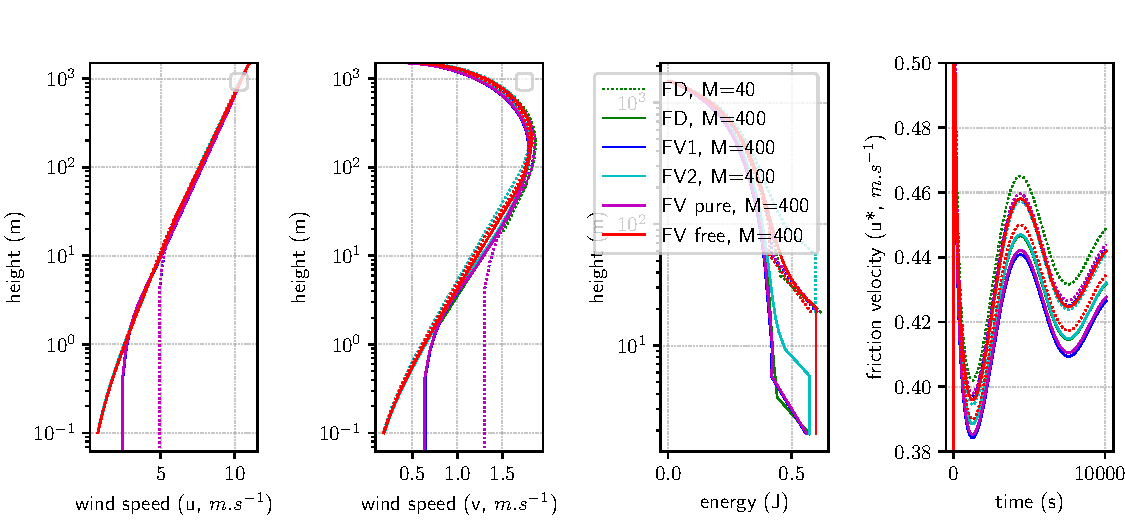
\includegraphics[scale=0.55]{images/consistency_comparison.pdf}
	\includegraphics[scale=0.55]{images/consistency_comparison_linearscale.pdf}
	\caption{Neutral case's numerical experiment. Top: log-scaled, bottom: linear-scaled}
	\label{fig:ND_NeutralCase_NumericalExp}
\end{figure}
\subsection{Variation of $\delta_{\rm sl}$}
In this subsection we assume that $\delta_{\rm sl}$ can differ
from one time to another. Let us note
$\delta_{\rm sl}^n, \delta_{\rm sl}^{n+1}$ the two different sizes
of the surface layer.
There are 3 cases to take into account:
\begin{enumerate}
\item there is a $k$ such that
	$z_k< \delta_{\rm sl}^n, \delta_{\rm sl}^{n+1} < z_{k+1}$
\item there is a $k$ such that
	$ \delta_{\rm sl}^n < z_k < \delta_{\rm sl}^{n+1}$
\item there is a $k$ such that
	$ \delta_{\rm sl}^n > z_k > \delta_{\rm sl}^{n+1}$
\end{enumerate}
Note that multiple grid levels can be between $\delta_{\rm sl}^{n}$
and $\delta_{\rm sl}^{n+1}$ in the second and third cases.
\par
Let $k^n$ be such that $z_{k^n} < \delta_{\rm sl}^{n}< z_{k^n + 1}$
and $k^{n+1}$ such that
$z_{k^{n+1}} < \delta_{\rm sl}^{n+1}< z_{k^{n+1} + 1}$
\begin{enumerate}
	\item $k^n = k^{n+1}$:
Since $\delta_{\rm sl}$ changes, then $\widetilde{h}$ also change.
It must be taken into account when
discretising in time the equations
\eqref{eq:ND_NeutralCase_prognosticEqFVfree} and 
\eqref{eq:ND_NeutralCase_semiDiscreteEkmanEqFVfree}.
The boundary condition stays \eqref{eq:ND_NeutralCase_boundaryCondFVfree}.
	\item $k^n < k^{n+1}$:
\eqref{eq:ND_NeutralCase_boundaryCondFVfree},
\eqref{eq:ND_NeutralCase_prognosticEqFVfree} and 
\eqref{eq:ND_NeutralCase_semiDiscreteEkmanEqFVfree} only need to
be satisfied between $z_{k^{n+1}}$ and $z_{k^{n+1}+1}$.
Hence, $\tau_{sl}(t^n)$ is set to 0.
	\item $k^n > k^{n+1}$:
\eqref{eq:ND_NeutralCase_prognosticEqFVfree} and 
\eqref{eq:ND_NeutralCase_semiDiscreteEkmanEqFVfree}
need to be satisfied in both cells.
{\color{red} It is not possible to do this in a natural way,
because using \eqref{eq:ND_NeutralCase_prognosticEqFVfree}
assumes the solution was a quadratic spline whereas it was actually
a log profile.
}
\end{enumerate}
